%% ------------------------------------------------------------------------- %%
\chapter{Hash Tables}
\label{cap:Hash Tables}

%% ------------------------------------------------------------------- %%
%\begin{itemize}
%\item Define hash table and its operations
%\item Open Addressing Strategies (Linear Probing, Quadratic Probing, ...)
%\item Chaining Strategy (Simple Chaining, Move-to-front ...)
%\item Load factor and resizing/rehashing the table
%\end{itemize}
%% ------------------------------------------------------------------- %%


Hash tables or hash maps is one of the most used applications of hash functions. It is actually so used in computer science that is almost impossible to talk about one without mentioning the other. This data structure consists in associating a \textit{key} to a \textit{value} in a table. That is, given a \textit{key}, it can retrieve the correct \textit{value} for it.

It is considered one of the possible (and one of the best) implementations of a dictionary. It has to implement the \textbf{INSERT}, \textbf{FIND} and \textbf{REMOVE} opreations, that can be accessed from outside the dictionary. It usually implements a lot of other private methods. 

This data structure is usually considered very useful among software engineers and computer scientists, although it usually has a linear worst case cost for retrieving, inserting and deleting a key-value pair. That is because it has a constant average cost for those operations.

Moreover, when talking about hash tables we have the problem of key collision, that is when two keys maps to the same hash value. As we saw in the previous chapter, collisions are more common than not, so collision resolution is a critical problem. To solve that problem, we have several techniques that envolves different tradeoffs. Those techniques are usually divided into two main categories, open addressing and separate chaining. Other problem to consider regarding this data structure is when to resize the hash table, to minimize the chance of collision and the use o memory. For this last one we usually consider a load factor, \( \alpha \), that is the ratio of keys with the available slots.

Also, hash tables can be easily abstracted to hash sets, that are commonly used to store a set of elements and check if an element is there. We can abstract that data structure to a hash table always with an empty value. Hash sets are one of the common ways to implement sets in programming languages, like unordered\_set from C++14.

It is also important to notice that hash tables have applications in different areas of computer science also, like compilers, caches and database indexing.


\begin{figure}[h!]
  \centering
  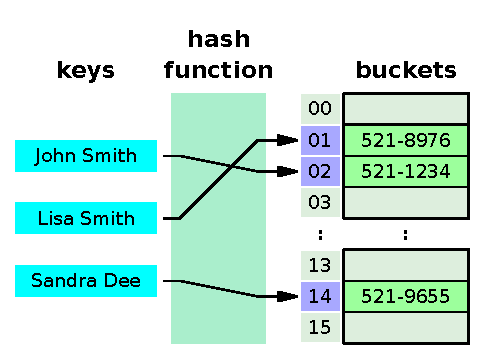
\includegraphics[width=12cm]{figuras/hash-table.pdf}
  \caption{Example of a hash table from string to string, more specifically name to number}
\end{figure}

\newpage

\section{Open Addressing}

\subsection{Implementing a no collision hash table}

To start I will give an example of a hash table that has a perfect hash function, that has no collisions. For that example we will use open addressing, that basically means that all data will be contained in an array. The operations \textbf{INSERT}, \textbf{FIND} and \textbf{REMOVE} would be very easy to imeplement. For the sake of simplicity, I will assume all the keys are strings. To start lets look at this simple class with dummy methods:

\begin{lstlisting}
class HashTable {
   vector< pair<string, int> > table;
   int m, n;
   
   HashTable() {
      m = 16;
      table.resize(m);
      n = 0;
   }

   unsigned int hashFunction(string s) {}
   
   void insert(string key, int value) {}

   int find(string key) {}

   void remove(string key) {}

private:
   double alpha = 1;
   void resizeIfNecessary() {}
}
\end{lstlisting}

As we can see it is pretty simple. The constructor builds a table of size \( 16 \), and we can assume a dinamic resizing every time the table is full. Later on we will see that this means that we resize every time the load factor, \( \alpha \), is equal to \( 1.00 \). We also can note that at the table part we are storing a pair of key and value, not just value. This is because we may want to retrieve all pairs of the table (like in a regular dictionary). The pairs are usually unordered (If they are not ordered by chance ...). We will skip the implementation of hashFunction, as we already saw plenty of it in the last chapter, so we will go right in for the implementation of \textbf{insert}:

\begin{lstlisting}
void insert(string key, int value) {
  unsigned int idx = hashFunction(key);
  table[idx] = pair<string, int>(key, value);
  n++;
  resizeIfNecessary();
}
\end{lstlisting}

That is pretty simple, that is mostly because we will assume that we will never have a collision, so we just put the key on the position returned by the hash function. The method \textbf{find} is implemented as following:

\begin{lstlisting}
int find(string key) {
  unsigned int idx = hashFunction(key);
  if (table[idx].first == key)
    return table[idx].second;
  return 0;
}
\end{lstlisting}

Also very simple, we always know the value will be in position returned by idx. The \textbf{remove} will be of the same simplicity, as following:

\begin{lstlisting}
void remove(string key) {
  unsigned int idx = hashFunction(key);
  table[idx].first = pair<string, int>("", 0);
  n--;
}
\end{lstlisting}

Here we make the assumption that an empty position has an empty string. We could also carry a boolean (usually called a tombstone) to check if the position is occupied or not. 

\subsection{Formal definition}

We can define open addressing in a general way as a hash table algorithm where the data always stay within the same vector. So, in the case of a collision, we need to define a sistematic way to traverse the table. The sequence of elements I need to traverse when I have a collision is called \textit{``Proble sequence''}. With that our hash function would change to the following:

\[ H(x, i) \]

Where \( x \) is our key and \( i \) is the sequence number. So every time we have a collision in \( H(x, i) \) we can simply go to \( H(x, i + 1) \). Given that, lets look into some different probe sequences.

\subsection{Linear Probing}

Linear probing is one of the most simple an practical probe sequences known. The probe sequence is basically:

\[ H(x, i) = (H(x) + i) \mod M \]

where \( M \) is the table size. That is a very simple probe sequence with not much secret on it. To implement the \textbf{insert} we can do the follwing:

\begin{lstlisting}
void insert(string key, int value) {
  unsigned int idx = hashFunction(key);
  while (table[idx] != pair<string, int>("", 0))
    idx = (idx + 1) % m;      
  table[idx] = pair<string, int>(key, value);
  n++;
  resizeIfNecessary();
}
\end{lstlisting}

That assumes that pair<string, int>("", 0) is the empty position, and performs a linear search until it finds one empty position to put the new (key, value) pair. The implementation of find \textbf{find} is very similar:

\begin{lstlisting}
int find(string key) {
  unsigned int idx = hashFunction(key);
  while (table[idx] != pair<string, int>("", 0)) {
    if (table[idx].first == key) 
      return table[idx].second;
    idx = (idx + 1) % m;
  }
  return 0;
}
\end{lstlisting}

It performs a linear search until it finds the element. If it does not find the element, it then returns a default value that in our case is 0. 

For removal, we have the problem that we cannot leave ``Holes'' in our table. That will be discussed more in depth later on the section ``How to delete an entry''. For now we will remove the elment, and shift the rest of the sequence one position. For that we can do the following:

\begin{lstlisting}
void remove(string key) {
  unsigned int idx = hashFunction(key);
  while (table[idx] != pair<string, int>("", 0)) {
    if (table[idx].first == key) 
      break;
      idx = (idx + 1) % m;
  }
    
  if (table[idx].first == key) {
    table[idx] = pair<string, int>("", 0);
    while (table[(idx + 1) % m] != pair<string, int>("", 0)) {
      swap(table[idx], table[idx + 1]);
      idx = (idx + 1) % m;
    }
    n--;
  }  
}
\end{lstlisting}

With that, the three operations have linear complexity. As we saw, we know hash functions that are considered good, with a rate of collision very close to an uniformly random function. Those functions will leave us with an expected constant time for those operations, and we will see later on that in practice it is much faster than linear access.

\subsection{Quadratic Probing}

\subsection{When to resize an array}

\subsection{How to delete an entry}

\section{Chaining Hashing}

Chaining hashing is the implementation of a hash table using a container, usally called bucket, to store the (key, value) pairs with a given hash. On this implementation, each bucket of the table is a linked list, that will carry the key value pair in our case. We deal with collisions with this implementation by adding a new node to the start of the list.

This implementation is considered simpler than open addressing, usually because the way of dealing with collisions is clearer. Also it is less system dependant if we consider performance (as we saw one of the key advantages of open addressing is that it is cache friendly). That is one of the key reasons that C++ uses chaining hashing for its default implementation of unordered\_hash \cite{HashTableProposal}.

Below we will discuss an implementation of chaining hashing in C++14:

\subsection{Simple Chaining Hashing Algorithm}

For this Chaining hashing implementation we will use C++14 STL data structure list as our container. list is a doubly linked list. For our \textbf{insert} we can implement it in the following way:

\begin{lstlisting}
void insert(string key, int value) {
  unsigned int idx = hashFunction(key);      
  table[idx].emplace_front(key, value);
  n++;
  resizeIfNecessary();
}
\end{lstlisting}

As we can see it is a very simple implementation, we just push a new element in the front of the list pointed in the idx. As before we add the counter of elements in the list and call resizeIfNcessary().

For \textbf{find} we can implement in the following way:

\begin{lstlisting}
int find(string key) {
  unsigned int idx = hashFunction(key);
  auto it = find_if(table[idx].begin(), table[idx].end(),
                    [&key](auto& kv) { return kv.first == key; });
  if (it != table[idx].end())
    return it->second;
  return 0;
}
\end{lstlisting}

That implementation is very succint but uses some of the features of C++14 (such as generic lambdas). For \textbf{erase} we can implement in a very similar fashion:

\begin{lstlisting}
void remove(string key) {
  unsigned int idx = hashFunction(key);
  auto it = find_if(table[idx].begin(), table[idx].end(),
                    [&key](auto& kv) { return kv.first == key; });
  if (it != table[idx].end()) {
    table[idx].erase(it);
    n--;
  }
}
\end{lstlisting}

As we can see, with linked list it is clearly easier to erase an element. 

\subsection{Move to front}

\subsection{When to resize an array}

\subsection{How to delete an entry}

\section{Open Addressing vs Chaining Hashing}

When comparing Open Addressing vs Chaning hashing we can cite many pros and cons. Lets start with the open addressing pros. Among the pros of open addressing we can see that open addressing techniques such as linear probing tend to be more cache friendly. That is because as the key value pairs are stored in the memory in a sequential way with the vector, when loading a key value pair we will load a chuck of memory that is around him (that will have other key value pairs). Another thing that can be said to ilustrate that is the 80 / 20 percent rule, that when applied to hash tables means that ``in practice'' 80\% of the keys will be accessed 20\% of the time (and 20\% of the keys will be accessed 80\% of the time). This is only for illustration purposes, obviously this is not valid for every application, as we can artificially create one that don't apply. Another advantage of open addressing is that all the memory will be in a single and sequential ``Block'' of memory. 